% Chapter 3: Project Development

\chapter{Desarrollo del Proyecto} % Main chapter title

\label{Chapter3} % For referencing this chapter elsewhere, use \ref{Chapter3}

%-------------------------------------------------------------------------------

\section{Trabajo previo}

Para entender el proceso de desarrollo que ha seguido este proyecto, es importante hacer un pequeño repaso al trabajo previo que se realizó en \nameref{sec:cauldron}\index{Cauldron} el cual, como se explicó en capítulos anteriores, motivó la realización de este proyecto.

\nameref{sec:cauldron}\index{Cauldron} nace con la idea de facilitar el uso de \nameref{sec:grimoirelab}\index{GrimoireLab}, y permitir usar este a perfiles no técnicos. Es por ello que el desarrollo de este \emph{SaaS} comienza como una aplicación web, utilizando \nameref{sec:django}\index{Django} como base y Elasticsearch\index{Elasticsearch} y Kibana\index{Kibana} para el manejo de datos. \nameref{sec:cauldron}\index{Cauldron} comienza en sus inicios con pocas fuentes de datos disponibles, únicamente Git\index{Git}, aunque muy temprano comienza a incluir otras muchas como GitHub\index{GitHub}, GitLab, o Meetup, entre otras.

\nameref{sec:cauldron}\index{Cauldron} está ideado para generar informes modificables. Esto quiere decir que un usuario puede, en un momento dado, solicitar el análisis de ciertas fuentes de datos, e.g., repositorios Git\index{Git}, y una vez terminado el análisis de esta incluir una nueva fuente de datos, como Meetup. Este esquema, si bien dota a la plataforma de mayor versatilidad, acarrea varios problemas en su desarrollo, ya que se necesitó realizar múltiples iteraciones en los modelos de la aplicación para conseguir que solo se analizaran las nuevas fuentes de datos, y no las ya analizadas.

\nameref{sec:cauldron}\index{Cauldron} hace uso de un sistema de \emph{workers} para realizar los análisis. Cada uno de estos \emph{workers} es un contenedor personalizado de \nameref{sec:grimoirelab}\index{GrimoireLab}, el cual es utilizado gracias a su SDK para \nameref{sec:python}\index{Python}. Estos \emph{workers} están ejecutando continuamente, y se establece su número al comienzo del despliegue del \emph{cluster}. Las tareas de análisis que estos \emph{workers} realizan son gestionadas por un complejo componente personalizado conocido como \emph{Cauldron Pool Scheduler}, el cual realiza una asignación de recursos de análisis equitativa entre todos los usuarios de la plataforma. A pesar de los buenos resultados que este sistema genera, añade una excesiva complejidad a la asignación de tareas, lo que ha dificultado realizar cualquier tipo de modificación a este en el pasado.

\begin{figure}[ht]
    \centering
    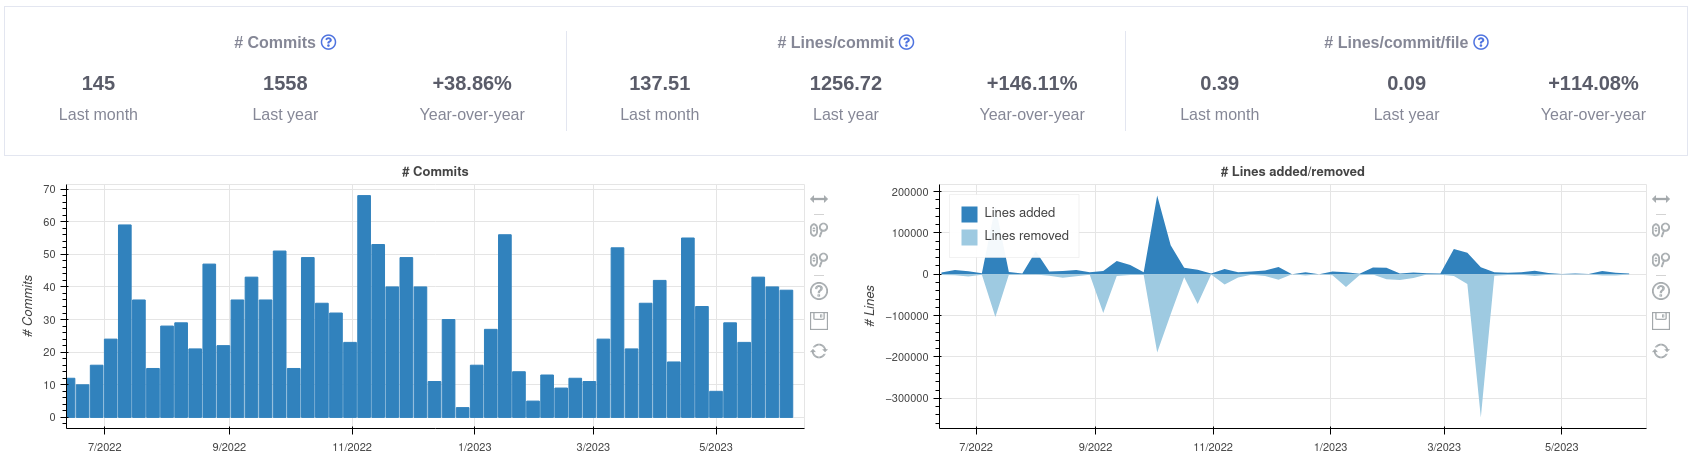
\includegraphics[width=\textwidth]{Figures/cauldron-metrics-charts}
    \decoRule
    \caption[Cauldron (Métricas)]{Métricas en Cauldron}
    \label{fig:cauldron-metrics-charts}
\end{figure}

Además de las métricas y gráficas que \nameref{sec:cauldron}\index{Cauldron} ofrece a través de Elasticsearch\index{Elasticsearch} y Kibana\index{Kibana}, existen otras muchas en la página de cada análisis (Figura~\ref{fig:cauldron-metrics-charts}). El desarrollo de estas métricas y gráficas, usando la librería \code{Bokeh} para JavaScript, no estuvo exento de dificultad. Debido a la gran cantidad de datos que algunos análisis manejan, en ocasiones la recogida de estos datos desde el \emph{cluster} de Elasticsearch\index{Elasticsearch} hacía vencer un \emph{timeout} establecido, lo que provocaba el fallo de la página. Además de esto, la inclusión de datos en las gráficas añadía una excesiva complejidad al código, haciendo difícil su modificación.

Estas y otras muchas situaciones originadas durante el desarrollo de \nameref{sec:cauldron}\index{Cauldron} (y su posterior mantenimiento) han resultado en un excelente valor didáctico, y han motivado varios de los objetivos que persigue este proyecto.

%-------------------------------------------------------------------------------

\section{Arquitectura del software}

El objetivo de este proyecto es proporcionar un servicio que permita analizar proyectos \emph{software}\index{software} de una manera sencilla y automatizada. Para ello, se ha llevado a cabo el desarrollo de varios prototipos:

\begin{itemize}
    \item El primer prototipo sienta las bases de la arquitectura de la aplicación. La API\index{API} consta de algunas llamadas básicas para la creación de solicitudes de análisis y el cliente es capaz de procesarlas y retornar este resultado al usuario.
    \item El segundo prototipo añade \nameref{sec:grimoirelab}\index{GrimoireLab} y \nameref{sec:opensearch}\index{OpenSearch} al esquema de la aplicación. La API\index{API} incluye nuevas estructuras y llamadas y el cliente ejecuta tareas de análisis con GrimoireLab y sube los resultados a OpenSearch para su visionado.
\end{itemize}

\subsection{Grimoirebots I}

El primer prototipo de la aplicación está creado utilizando el framework \nameref{sec:drf}\index{Django} para \nameref{sec:python}\index{Python}, y \nameref{sec:poetry}\index{Poetry} como gestor de paquetes y dependencias. Esta primera versión establece la arquitectura base de la aplicación y el esquema de comunicación entre servidor y cliente.

Para este fin, se han desarrollado los siguientes modelos\footnote{Los campos no obligatorios aparecen coloreados en gris.}:

\begin{figure}[ht]
    \centering
    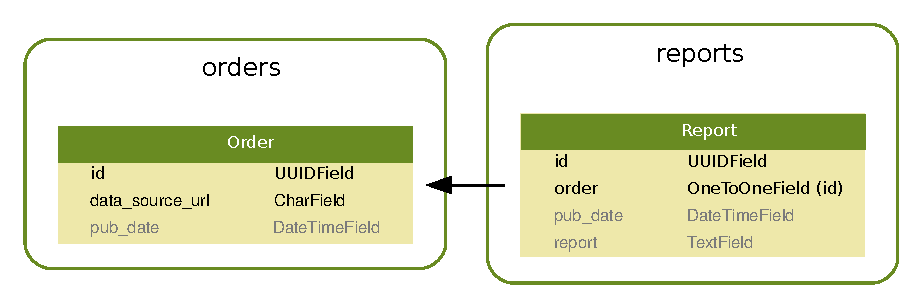
\includegraphics[width=0.8\textwidth]{Figures/grimoirebots_i_models}
    \decoRule
    \caption[Grimoirebots I (modelos)]{Modelos usados en Grimoirebots (Versión 1)}
    \label{fig:grimoirebots_i_models}
\end{figure}

\begin{itemize}
    \item \code{Order} -- Este modelo representa la solicitud hecha por un usuario. Está formado por un identificador UUID único, un \emph{string} representando la URL del repositorio git\index{Git} que se quiere analizar, y la fecha de creación de la instancia con un campo \emph{datetime}. (Figura~\ref{fig:grimoirebots_i_models})
    \item \code{Report} -- Este modelo representa el resultado de procesar una solicitud hecha por un usuario. Está formado por un identificador UUID único, una referencia a la solicitud (\code{Order}) que originó su creación, la fecha de creación de la instancia con un campo \emph{datetime}, y un \emph{string} representando el procesamiento de la solicitud. (Figura~\ref{fig:grimoirebots_i_models})
\end{itemize}

También se han desarrollado los siguientes \emph{paths} en la API\index{API}:

\begin{figure}[ht]
    \centering
    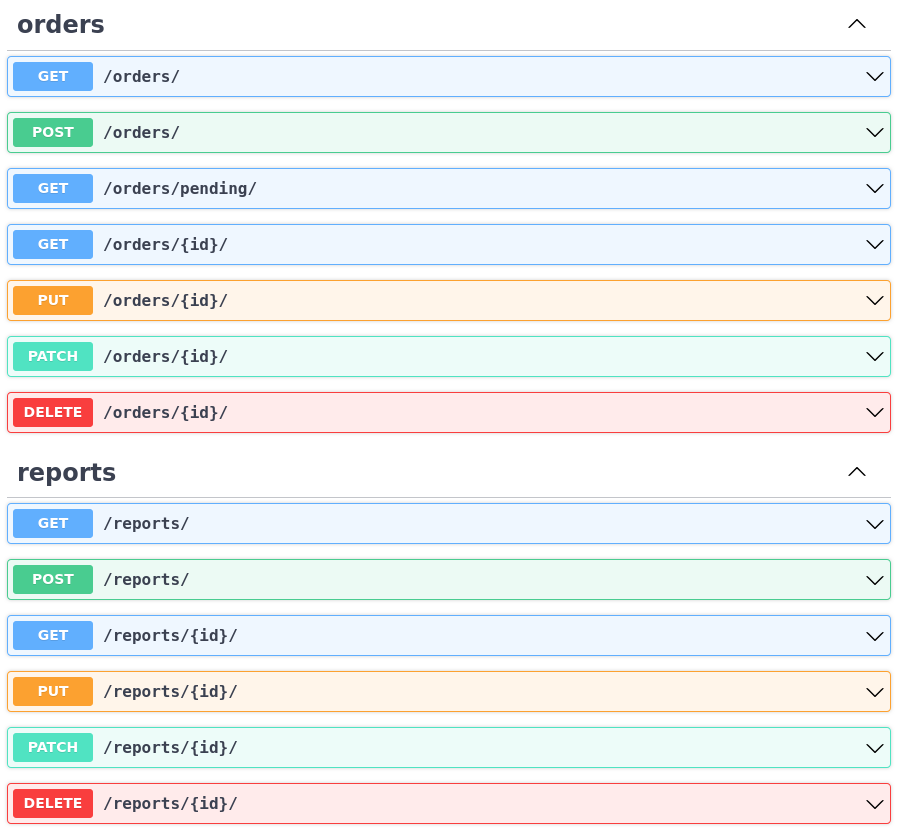
\includegraphics[width=0.8\textwidth]{Figures/grimoirebots_i_api}
    \decoRule
    \caption[Grimoirebots I (API)]{API de Grimoirebots (Versión 1)}
    \label{fig:grimoirebots_i_api}
\end{figure}

\begin{itemize}
    \item En la \emph{app} \code{orders} se han incluido \emph{paths} que permiten obtener la lista de solicitudes, la lista de solicitudes pendientes, y crear, modificar y eliminar solicitudes. (Figura~\ref{fig:grimoirebots_i_api})
    \item En la \emph{app} \code{reports} se han incluido llamadas para listar informes, y para crear, modificar y eliminar los mismos. (Figura~\ref{fig:grimoirebots_i_api})
\end{itemize}

Adicionalmente, se ha creado una imagen \nameref{sec:docker}\index{Docker} que instala las dependencias del proyecto y lo lanza utilizando \nameref{sec:gunicorn}\index{Gunicorn} como servidor WSGI, y se ha incluido el uso de \nameref{sec:dependabot}\index{Dependabot} para la comprobación de cualquier actualización en las dependencias del proyecto y avisar de esto al equipo desarrollador.

Por otra parte, el cliente o bot automático es una aplicación escrita en \nameref{sec:python}\index{Python} que, haciendo uso de la librería \code{apiclient}, recoge periódicamente aquellas solicitudes pendientes de procesar y realiza un procesamiento básico de ellas. En esta parte del desarrollo aún no se había incluido \nameref{sec:grimoirelab}\index{GrimoireLab}, por lo que el procesamiento que el cliente hace de la solicitud es la construcción de un \emph{string} que contiene el identificador y el repositorio de la solicitud.

Para ilustrar el comportamiento de este prototipo, se han creado las siguientes infografías:

\begin{figure}[ht]
    \centering
    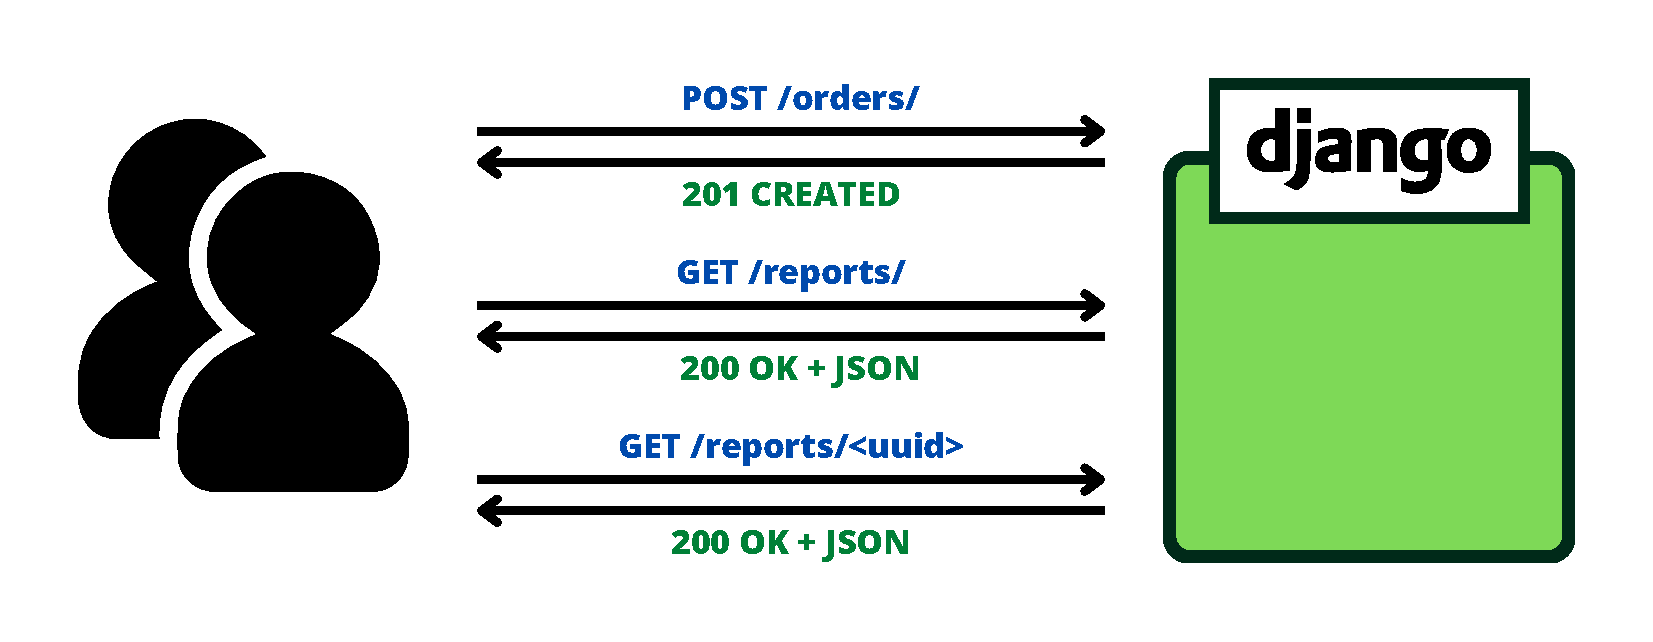
\includegraphics[width=0.8\textwidth]{Figures/grimoirebots_frontend}
    \decoRule
    \caption[Grimoirebots (\emph{Frontend})]{\emph{Frontend} de Grimoirebots (Versiones 1 y 2)}
    \label{fig:grimoirebots_frontend}
\end{figure}

Como muestra la Figura~\ref{fig:grimoirebots_frontend}, el usuario crea nuevas solicitudes de análisis realizando una llamada POST a \code{/orders/}. El usuario puede listar los informes creados mediante una llamada GET a \code{/reports/} y acceder a cada uno de ellos mediante una llamada GET a \code{/reports/<uuid>}.

\begin{figure}[ht]
    \centering
    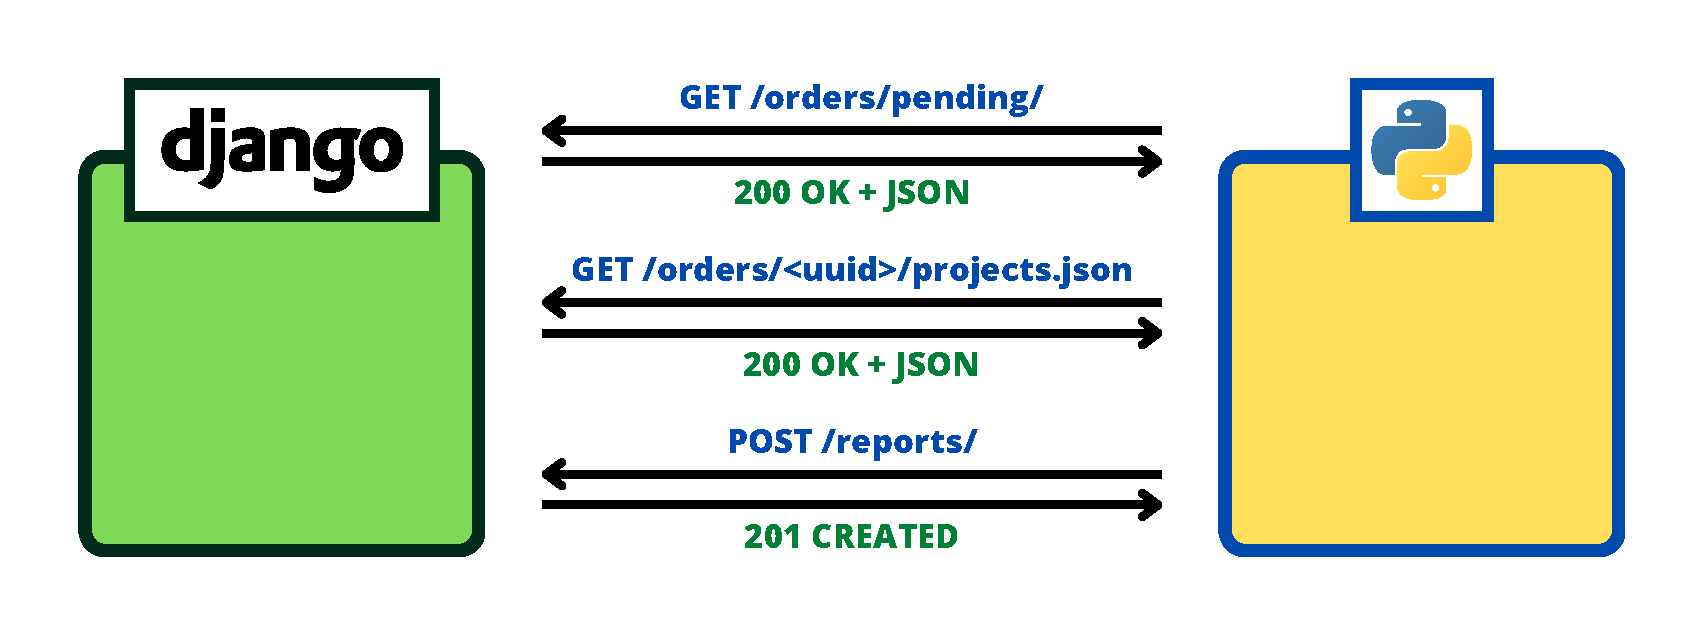
\includegraphics[width=0.8\textwidth]{Figures/grimoirebots_i_backend}
    \decoRule
    \caption[Grimoirebots I (\emph{Backend})]{\emph{Backend} de Grimoirebots (Versión 1)}
    \label{fig:grimoirebots_i_backend}
\end{figure}

Por su parte, en la Figura~\ref{fig:grimoirebots_i_backend} se incluyen las interacciones que realiza el cliente con la API\index{API} para procesar las solicitudes de los usuarios. Periódicamente, el cliente pide al servidor las solicitudes que aún no hayan sido procesadas. Por cada una de estas, pide el repositorio solicitado para analizar haciendo una llamada GET a \code{/orders/<uuid>/projects.json}. Posteriormente, realiza el procesamiento básico comentado anteriormente y realiza una llamada POST a \code{/reports/} para crear el informe y asociarlo con la solicitud del usuario.

\subsection{Grimoirebots II}

El segundo (y último) prototipo utiliza las mismas tecnologías mencionadas en el prototipo anterior, y algunas añadidas. Como gran aditivo, en este prototipo se incluye el uso de \nameref{sec:grimoirelab}\index{GrimoireLab} y \nameref{sec:opensearch}\index{OpenSearch} para realizar el análisis de proyectos \emph{software}\index{Software}.

Debido a esto, este prototipo actualiza los modelos de la aplicación de la siguiente forma\footnote{Igual que en el apartado anterior, los campos no obligatorios aparecen coloreados en gris.}:

\begin{figure}[ht]
    \centering
    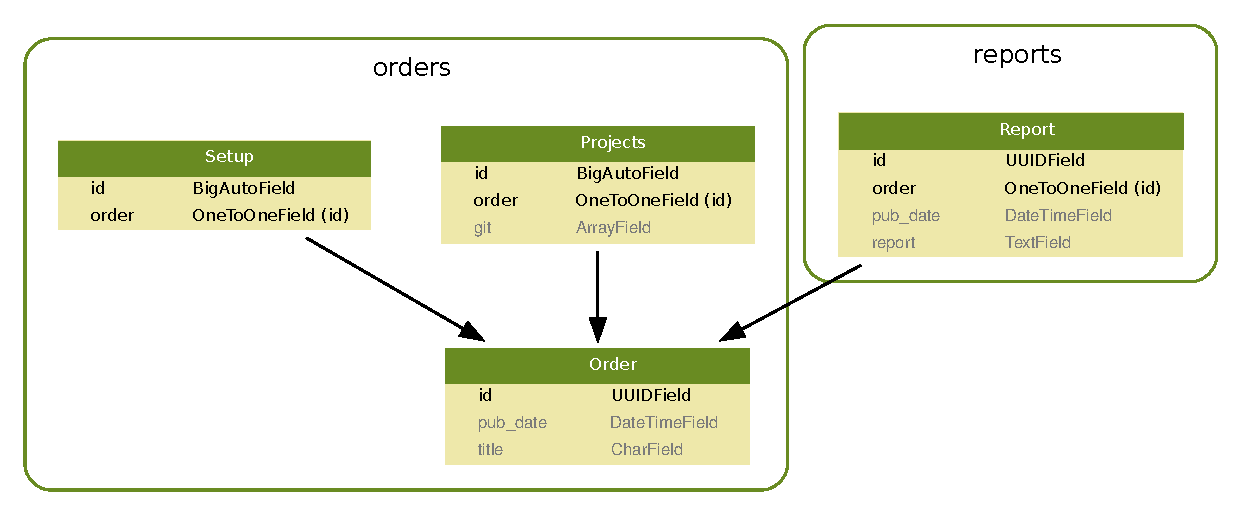
\includegraphics[width=0.8\textwidth]{Figures/grimoirebots_ii_models}
    \decoRule
    \caption[Grimoirebots II (modelos)]{Modelos usados en Grimoirebots (Versión 2)}
    \label{fig:grimoirebots_ii_models}
\end{figure}

\begin{itemize}
    \item \code{Order} -- Este modelo sigue representando la solicitud hecha por un usuario. El campo \code{data\_source\_url} ha sido eliminado y se ha incluido un campo \code{title} para que el usuario pueda identificar más fácilmente la solicitud. (Figura~\ref{fig:grimoirebots_ii_models})
    \item \code{Setup} -- Este modelo representa la configuración utilizada por \nameref{sec:grimoirelab}\index{GrimoireLab} en el análisis de proyectos \emph{software}\index{Software}. Está enlazado con una solicitud específica mediante el campo \code{order}. (Figura~\ref{fig:grimoirebots_ii_models})
    \item \code{Projects} -- Este modelo representa la lista de repositorios git\index{Git} que un usuario ha solicitado analizar. Está compuesto por un identificador numérico único, el identificador de la solicitud, y una lista de \emph{strings} con las URLs de los repositorios. (Figura~\ref{fig:grimoirebots_ii_models})
    \item \code{Report} -- Este modelo no ha sufrido cambios en este prototipo. (Figura~\ref{fig:grimoirebots_ii_models})
\end{itemize}

Los \emph{paths} que incluye la API\index{API} de este prototipo son los mismos que en el anterior, a excepción de:

\begin{figure}[ht]
    \centering
    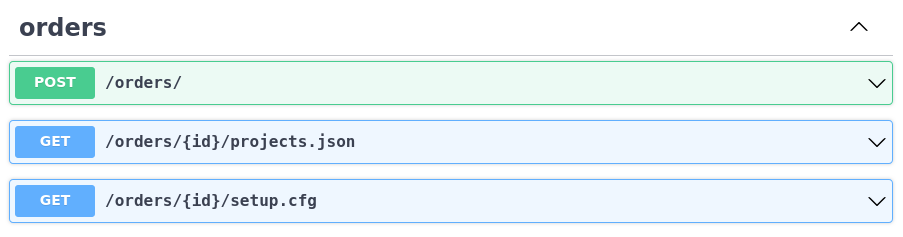
\includegraphics[width=0.8\textwidth]{Figures/grimoirebots_ii_api}
    \decoRule
    \caption[Grimoirebots II (API)]{API de Grimoirebots (Versión 2)}
    \label{fig:grimoirebots_ii_api}
\end{figure}

\begin{itemize}
    \item La llamada POST a \code{/orders/} ahora incluye los campos \code{title}, \code{projects}, y \code{setup} en el cuerpo de la petición. De esta forma, el usuario utiliza una única llamada para crear su solicitud de análisis. (Figura~\ref{fig:grimoirebots_ii_api})
    \item Se han incluido las llamadas GET para \code{/orders/<uuid>/projects.json} y para \code{/orders/<uuid>/setup.cfg} para obtener los ficheros con la lista de repositorios y la configuración para \nameref{sec:grimoirelab}\index{GrimoireLab}, respectivamente. (Figura~\ref{fig:grimoirebots_ii_api})
\end{itemize}

El cliente es modificado en este prototipo para incluir el uso de \nameref{sec:grimoirelab}\index{GrimoireLab}. La forma en que el cliente hace uso de esta herramienta es mediante un contenedor \nameref{sec:docker}\index{Docker}\footnote{\url{https://hub.docker.com/r/grimoirelab/grimoirelab}} lanzado desde el mismo cliente gracias a la librería \code{docker}.

Por otro lado, en este prototipo se incluye el uso de \nameref{sec:opensearch}\index{OpenSearch} y OpenSearch Dashboards para almacenar y visionar los datos generados por \nameref{sec:grimoirelab}\index{GrimoireLab}. Este sistema es lanzado mediante \nameref{sec:docker}\index{Docker} Compose\footnote{Docker Compose es una herramienta que permite lanzar múltiples contenedores de manera simultánea, mediante ficheros de configuración.}, y se ha construido un fichero de configuración con las características que necesita el sistema.

Igual que en el prototipo anterior, se han creado algunas infografías para ilustrar su comportamiento:

En el caso de la interacción entre usuario y servidor, el comportamiento es el mismo que en el prototipo 1. (Véase~\ref{fig:grimoirebots_frontend})

\begin{figure}[ht]
    \centering
    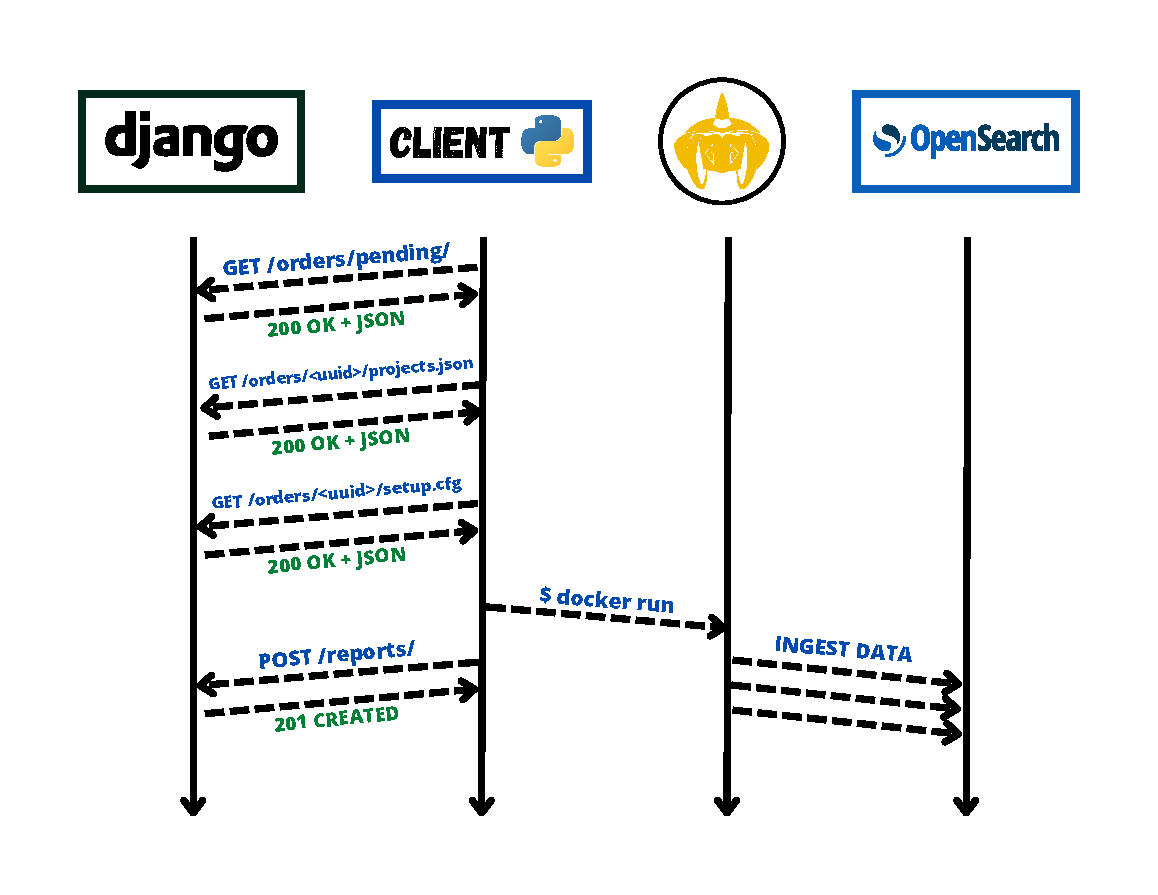
\includegraphics[width=0.8\textwidth]{Figures/grimoirebots_ii_backend}
    \decoRule
    \caption[Grimoirebots II (\emph{Backend})]{\emph{Backend} de Grimoirebots (Versión 2)}
    \label{fig:grimoirebots_ii_backend}
\end{figure}

El \emph{backend}, sin embargo, sufre varios cambios. Como muestra la Figura~\ref{fig:grimoirebots_ii_backend}, el cliente obtiene la lista de solicitudes pendientes. Para cada una de ellas obtiene los ficheros de repositorios y configuración. A continuación, utiliza la librería \code{docker} para lanzar un contenedor de \nameref{sec:grimoirelab}\index{GrimoireLab} por cada solicitud, incluyendo los ficheros antes mencionados en el volumen que utiliza cada contenedor. Por último, cada contenedor realizará el análisis de los repositorios indicados en la solicitud e ingestará los datos al \emph{cluster} de \nameref{sec:opensearch}\index{OpenSearch}, desde donde el usuario es capaz de operar con ellos.

%-------------------------------------------------------------------------------

\section{Problemas encontrados}

Durante el desarrollo del proyecto, surgieron algunas situaciones que dificultaron la finalización del mismo.

En una etapa temprana del desarrollo se pensó en incluir usuarios en la plataforma, cada uno de ellos con acceso únicamente a sus informes, gráficas y visualizaciones. Esto, añadido a la necesidad de incluir mecanismos de autenticación a la API\index{API}, supuso añadir demasiada complejidad al proyecto y fue descartado por este motivo.

Se quiso utilizar, al comienzo, la versión estándar de \nameref{sec:django}\index{Django} incluyendo su sistema de \emph{templates}. Esto era debido a que la aplicación contaba en un principio con un \emph{frontend} con interfaz gráfica, la cual sería accesible desde un navegador web. Debido a las ventajas que suponía el uso de \nameref{sec:drf} (como el uso de \emph{serializers}) se decidió utilizar este para parte del \emph{backend}. Sin embargo, este módulo funcionaba de manera bastante mala con el sistema de templates de \nameref{sec:django}. Finalmente, se decidió continuar usando \nameref{sec:drf} y dejar de lado la interfaz gráfica.

Uno de los ficheros que \nameref{sec:grimoirelab}\index{GrimoireLab} utiliza, el llamado fichero de configuración, utiliza un formato con una estructura muy similar al que puede encontrarse en los ficheros INI usados en Microsoft Windows. Este formato no es soportado de forma nativa por \nameref{sec:drf}, y causó varios retrasos tratando de implementar una solución para hacerlo viable. Finalmente, y con el fin de sacar el proyecto adelante, se decidió hacer que la API\index{API} devolviera el fichero con formato JSON\index{JSON} y luego, en el cliente, convertir este al formato necesario usando la librería \code{configparser}. Esto fue posible debido a que ambos formatos comparten similitudes que hacen viable su conversión.

Durante la última etapa del desarrollo, se quiso incluir una versión de Grimoirebots desarrollada con \nameref{sec:fastapi}\index{FastAPI}, con el fin de comparar este con \nameref{sec:drf}. Sin embargo, este prototipo nunca llegó a ver la luz por falta de tiempo, aunque se realizaron algunas pruebas que pueden encontrarse en \nameref{sec:github}\index{GitHub}\footnote{\url{https://github.com/merinhunter/grimoirebots-fastapi}}.

Además de todo lo anterior, existieron otros pequeños problemas que ralentizaron el desarrollo del proyecto, como el intento de incluir paginación, la complejidad de ejecutar contenedores\index{Contenedor} desde otro contenedor, o la falta de documentación en algunos módulos de \nameref{sec:grimoirelab}. Sin embargo, todos estos incidentes tienen un alto valor didáctico, y su documentación permitirá no volver a cometerlos en el futuro.
